\documentclass{article} % A4 paper and 11pt font size
\setcounter{secnumdepth}{0}

\usepackage{amssymb, amsmath, amsfonts}
\usepackage{moreverb}
\usepackage{graphicx}
\usepackage{enumerate}
\usepackage{graphics}
\usepackage[margin=1.25in]{geometry}
\usepackage{color}
\usepackage{tocloft}
\renewcommand{\cftsecleader}{\cftdotfill{\cftdotsep}}
\usepackage{array}
\usepackage{float}
\usepackage{hyperref}
\usepackage{textcomp}
\usepackage[makeroom]{cancel}
\usepackage{bbold}
\usepackage{alltt}
\usepackage{physics}
\usepackage{mathtools}
\usepackage[normalem]{ulem}
\usepackage{amsthm}
\usepackage{tikz}
\usetikzlibrary{positioning}
\usetikzlibrary{arrows}
\usepackage{pgfplots}
\usepackage{bigints}
\allowdisplaybreaks
\pgfplotsset{compat=1.12}

\theoremstyle{plain}
\newtheorem*{theorem*}{Theorem}
\newtheorem{theorem}{Theorem}
\newtheorem*{lemma*}{Lemma}
\newtheorem{lemma}{Lemma}

\newenvironment{definition}[1][Definition]{\begin{trivlist}
\item[\hskip \labelsep {\bfseries #1}]}{\end{trivlist}}

\newcommand{\E}{\varepsilon}
\def\Rl{\mathbb{R}}
\def\Cx{\mathbb{C}}

\newcommand{\Ei}{\text{Ei}}

\usepackage[T1]{fontenc} % Use 8-bit encoding that has 256 glyphs
\usepackage{fourier} % Use the Adobe Utopia font for the document - comment this line to return to the LaTeX default
\usepackage[english]{babel} % English language/hyphenation

\usepackage{sectsty} % Allows customizing section commands
\allsectionsfont{\centering \normalfont\scshape} % Make all sections centered, the default font and small caps

\usepackage{fancyhdr} % Custom headers and footers
\pagestyle{fancy} % Makes all pages in the document conform to the custom headers and footers
\fancyhead[L]{\bf Sam Fleischer}
\fancyhead[C]{\bf UC Davis \\ Applied Mathematics (MAT207C)} % No page header - if you want one, create it in the same way as the footers below
\fancyhead[R]{\bf Spring 2016}

\fancyfoot[L]{\bf } % Empty left footer
\fancyfoot[C]{\bf \thepage} % Empty center footer
\fancyfoot[R]{\bf } % Page numbering for right footer
\renewcommand{\headrulewidth}{0pt} % Remove header underlines
\renewcommand{\footrulewidth}{0pt} % Remove footer underlines
\setlength{\headheight}{25pt} % Customize the height of the header

\newcommand{\VEC}[2]{\left\langle #1, #2 \right\rangle}
\newcommand{\ran}{\text{\rm ran }}
\newcommand{\Hilb}{\mathcal{H}}
\newcommand{\lap}{\Delta}

\DeclareMathOperator*{\esssup}{\text{ess~sup}}

\newcommand{\problem}[2]{
\vspace{.375cm}
\boxed{\begin{minipage}{\textwidth}
    \section{\bf #1}
    #2
\end{minipage}}
}

\numberwithin{equation}{section} % Number equations within sections (i.e. 1.1, 1.2, 2.1, 2.2 instead of 1, 2, 3, 4)
\numberwithin{figure}{section} % Number figures within sections (i.e. 1.1, 1.2, 2.1, 2.2 instead of 1, 2, 3, 4)
\numberwithin{table}{section} % Number tables within sections (i.e. 1.1, 1.2, 2.1, 2.2 instead of 1, 2, 3, 4)

\setlength\parindent{0pt} % Removes all indentation from paragraphs - comment this line for an assignment with lots of text

\newcommand{\horrule}[1]{\rule{\linewidth}{#1}} % Create horizontal rule command with 1 argument of height

\usepackage{xcolor}
\definecolor{light-gray}{gray}{0.9}

\title{ 
\normalfont \normalsize 
\textsc{UC Davis, Applied Mathematics (MAT207C), Spring 2016} \\ [25pt] % Your university, school and/or department name(s)
\horrule{2pt} \\[0.4cm] % Thin top horizontal rule
\Huge Homework \#3 \\ % The assignment title
\horrule{2pt} \\[0.5cm] % Thick bottom horizontal rule
}

\author{\huge Sam Fleischer} % Your name

\date{April 22, 2016} % Today's date or a custom date

\begin{document}\thispagestyle{empty}

\maketitle % Print the title

\makeatletter
\@starttoc{toc}
\makeatother

\pagebreak

%%%%%%%%%%%%%%%%%%%%%%%%%%%%%%%%%%%%%%
\problem{Problem 1}{In class we constructed the leading order composite expansion to the initial value problem
\begin{align*}
    \E\ddot{u} + \dot{u} + u &= 0, \\
    u(0) = 0,\qquad \E&\dot{u}(0) = 1.
\end{align*}
\begin{enumerate}[(a)]
    \item Find the terms at order $\E$ for the inner and outer expansions, perform matching at this order using the intermediate scale, and give the composite expansion.
    \item Compute the exact solution to this problem.  Use it to assess the accuracy of the leading order composite expansion and the expansion from part (a) for different values of $\E$.
\end{enumerate}}
\begin{proof}
    First, we compute the outer solution.  Since the layer is located at $0$, none of the boundary condtions apply.  Let $u = u_0 + \E u_1 + \E u_2^2 + \dots$ and let $\E \rightarrow 0$.  Then combine terms of similar order:
    \begin{align*}
        \dot{u}_0 + u_0 &= 0 \\
        \dot{u}_1 + u_1 &= -\ddot{u}_0 \\
        \dot{u}_2 + u_2 &= -\ddot{u}_1 \\
        &\vdots
    \end{align*}
    The general forms of the solutions are
    \begin{align*}
        u_0 = Ae^{-t} \qquad \text{and} \qquad u_1 = Be^{-t} - Ate^{-t}.
    \end{align*}
    Next, denote $\tau = \frac{t}{\E}$ and $U(\tau) = u(t)$.  This yields the following inner layer problem (where the boundary conditions apply):
    \begin{align*}
        \begin{cases}
            \ddot{U} + \dot{U} + \E U = 0 \\
            U(0) = 0 \\
            \dot{U}(0) = 1
        \end{cases}
    \end{align*}
    Then let $U = U_0 + \E U_1 + \E^2 U_2 + \dots$.  Combining terms of similar order gives
    \begin{align*}
        &\begin{cases}
            \ddot{U}_0 + \dot{U}_0 = 0 \\
            U_0(0) = 0 \\
            \dot{U}_0(0) = 1
        \end{cases}\\
        &\begin{cases}
            \ddot{U}_1 + \dot{U}_1 = -U_0 \\
            U_1(0) = 0 \\
            \dot{U}_1(0) = 0
        \end{cases} \\
        &\vdots
    \end{align*}
    Thus, $U_0(\tau) = 1 - e^{-\tau}$, which subsequentally yields $U_1(\tau) = -\tau\qty(1 + e^{-\tau}) + 2\qty(1 - e^{-\tau})$.  Thus,
    \begin{align*}
        u_{\text{out}}(t) &= Ae^{-t} + \E\qty(Be^{-t} - Ate^{-t}) \\
        u_{\text{in}}(t) &= \qty(1 - e^{-\frac{t}{\E}}) + \E\qty(-\frac{t}{\E}\qty(1 + e^{-\frac{t}{\E}}) + 2\qty(1 - e^{-\frac{t}{\E}})) \\
        &= \qty[1 - e^{-\frac{t}{\E}} - t\qty(1 + e^{-\frac{t}{\E}})] + 2\E\qty[1 - e^{-\frac{t}{\E}}]
    \end{align*}
    Obviously these don't simply match up, i.e.~$A$ and $B$ are not easily determined.  So we need to create an intermediate time scale $t_\eta = \frac{t}{\eta}$, such that $\E \prec \eta \prec 1$.  We want to match terms such that $u_\text{in}$ and $u_\text{out}$ match up to order $\E$.  So, we want to consider $0 = \displaystyle\lim_{\E \rightarrow 0}\qty[\frac{u_\text{in}(\eta t_\eta) - u_\text{out}(\eta t_\eta)}{\E}]$.
    \begin{align*}
        0 &= \lim_{\E \rightarrow 0}\frac{1}{\E}\qty(\qty[1 - e^{-\frac{\eta t_\eta}{\E}} - \eta t_\eta\qty(1 + e^{-\frac{\eta t_\eta}{\E}})] + 2\E\qty[1 - e^{-\frac{\eta t_\eta}{\E}}] - Ae^{-\eta t_\eta} - \E\qty(Be^{-\eta t_\eta} - A\eta t_\eta e^{-\eta t_\eta})) \\
        &= \lim_{\E \rightarrow 0}\frac{1}{\E}\qty(\qty[1 - e^{-\frac{\eta t_\eta}{\E}} - \eta t_\eta\qty(1 + e^{-\frac{\eta t_\eta}{\E}}) - A e^{-\eta t_\eta}] + \E\qty[2\qty(1 - e^{-\frac{\eta t_\eta}{\E}}) - B e^{-\eta t_\eta} + A\eta t_\eta e^{-\eta t_\eta}]) \\
        &= \lim_{\E \rightarrow 0} \qty[\frac{1}{\E} - \frac{1}{\E}\exp[-\frac{\eta t_\eta}{\E}] - \frac{\eta}{\E}t_\eta - \frac{\eta}{\E}t_\eta \exp[-\frac{\eta t_\eta}{\E}] - \frac{A}{\E}e^{-\eta t_\eta} + 2 - 2\exp[-\frac{\eta t_\eta}{\E}] - B e^{-\eta t_\eta} + A\eta t_\eta e^{-\eta t_\eta}]
    \end{align*}
    We neglect the transcendentally small terms (terms containing $\exp[-\frac{\eta t_\eta}{\E}]$).
    \begin{align*}
        0 &= \lim_{\E \rightarrow 0} \qty[\frac{1}{\E} - \frac{\eta}{\E}t_\eta - \frac{A}{\E}e^{-\eta t_\eta} + 2 - B e^{-\eta t_\eta} + A\eta t_\eta e^{-\eta t_\eta}]
    \end{align*}
    Note that since $\E \rightarrow 0$ then $\eta \rightarrow 0$ since $\E \prec \eta \prec 1$.  Next we employ Taylor expansions of $e^{-\eta t_\eta}$.
    \begin{align*}
        0 &= \lim_{\E \rightarrow 0} \Bigg[\frac{1}{\E}\qty(1 - A\qty[1 - \eta t_\eta + \frac{1}{2}\qty(\eta t_\eta)^2 + \dots]) + \qty(2 - B\qty[1 - \eta t_\eta + \frac{1}{2}(\eta t_\eta)^2 + \dots]) - \frac{\eta}{\E}t_\eta \\
        &\qquad \qquad + A\eta t_\eta\qty[1 - \eta t_\eta + \frac{1}{2} (\eta t_\eta)^2 + \dots]\Bigg]
    \end{align*}
    Assuming $\eta^2 \prec \E$, then $\frac{\eta^2}{\E} \rightarrow 0$, and so
    \begin{align*}
        \frac{1}{\E} - \frac{A}{\E} = 0 \qquad \text{and} \qquad 2 - B = 0 \qquad \implies \qquad A = 1 \qquad \text{and} \qquad B = 2.
    \end{align*}
    Thus,
    \begin{align*}
        u_{\text{out}}(t) &= e^{-t} + \E\qty(2e^{-t} - te^{-t}) \\
        u_{\text{in}}(t) &= \qty[1 - e^{-\frac{t}{\E}} - t\qty(1 + e^{-\frac{t}{\E}})] + 2\E\qty[1 - e^{-\frac{t}{\E}}]
    \end{align*}
    Finally, the composite expansion for this problem is
    \begin{align*}
        u(t) &= u_{\text{out}}(t) + u_{\text{in}}(t) - u_{\text{match}}(t) \\
        &= \underbrace{e^{-t} + \E\qty(2e^{-t} - te^{-t})}_{\text{outer layer expasion}} + \underbrace{\qty[1 - e^{-\frac{t}{\E}} - t\qty(1 + e^{-\frac{t}{\E}})] + 2\E\qty[1 - e^{-\frac{t}{\E}}]}_{\text{inner layer expansion}} - \underbrace{\qty[1 - t + 2\E]}_{\text{matched terms}}\\
        &= \qty[e^{-t} - (1 + t)e^{-\frac{t}{\E}}] + \E\qty[(2 - t)e^{-t} - 2e^{-\frac{t}{\E}}].
    \end{align*}
    Figures (\ref{problem_1_graphs}) and (\ref{problem_1_graphs_errors}) depicts the accuracy of the expansion for various values of $\E$.
    \begin{figure}
        \centering
        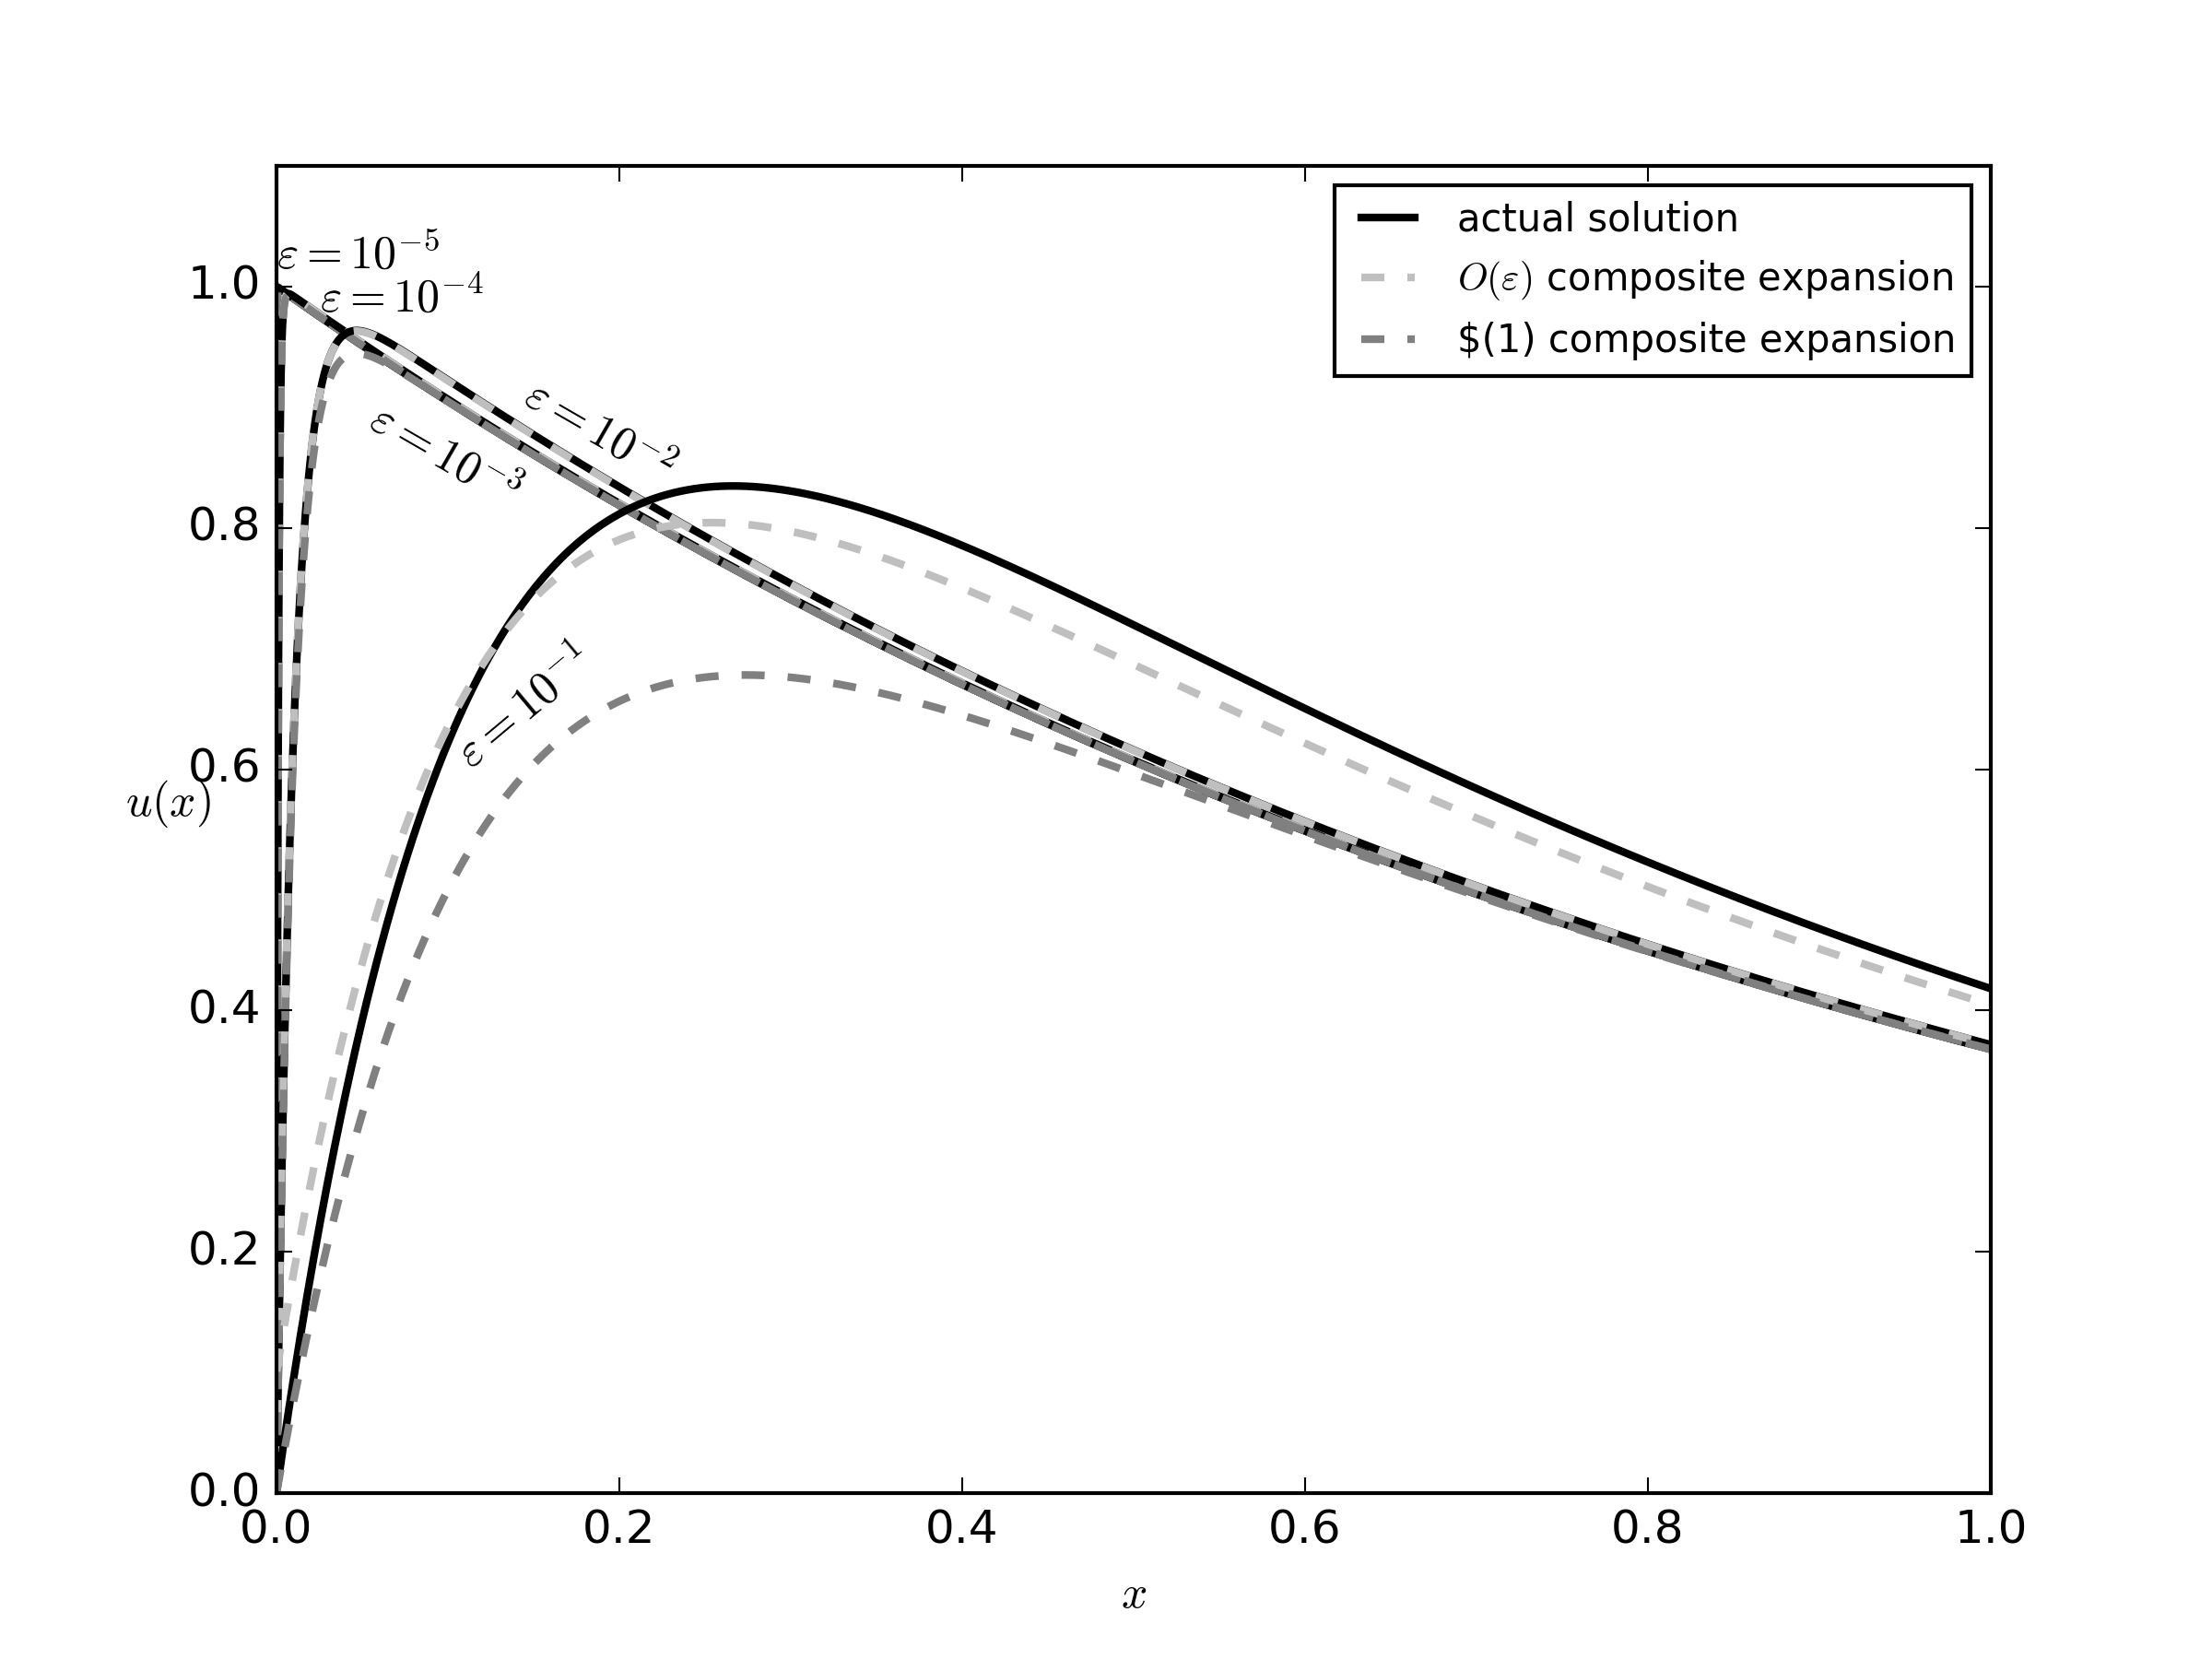
\includegraphics[width=0.75\textwidth]{standard.png}\vspace{-0.22cm}
        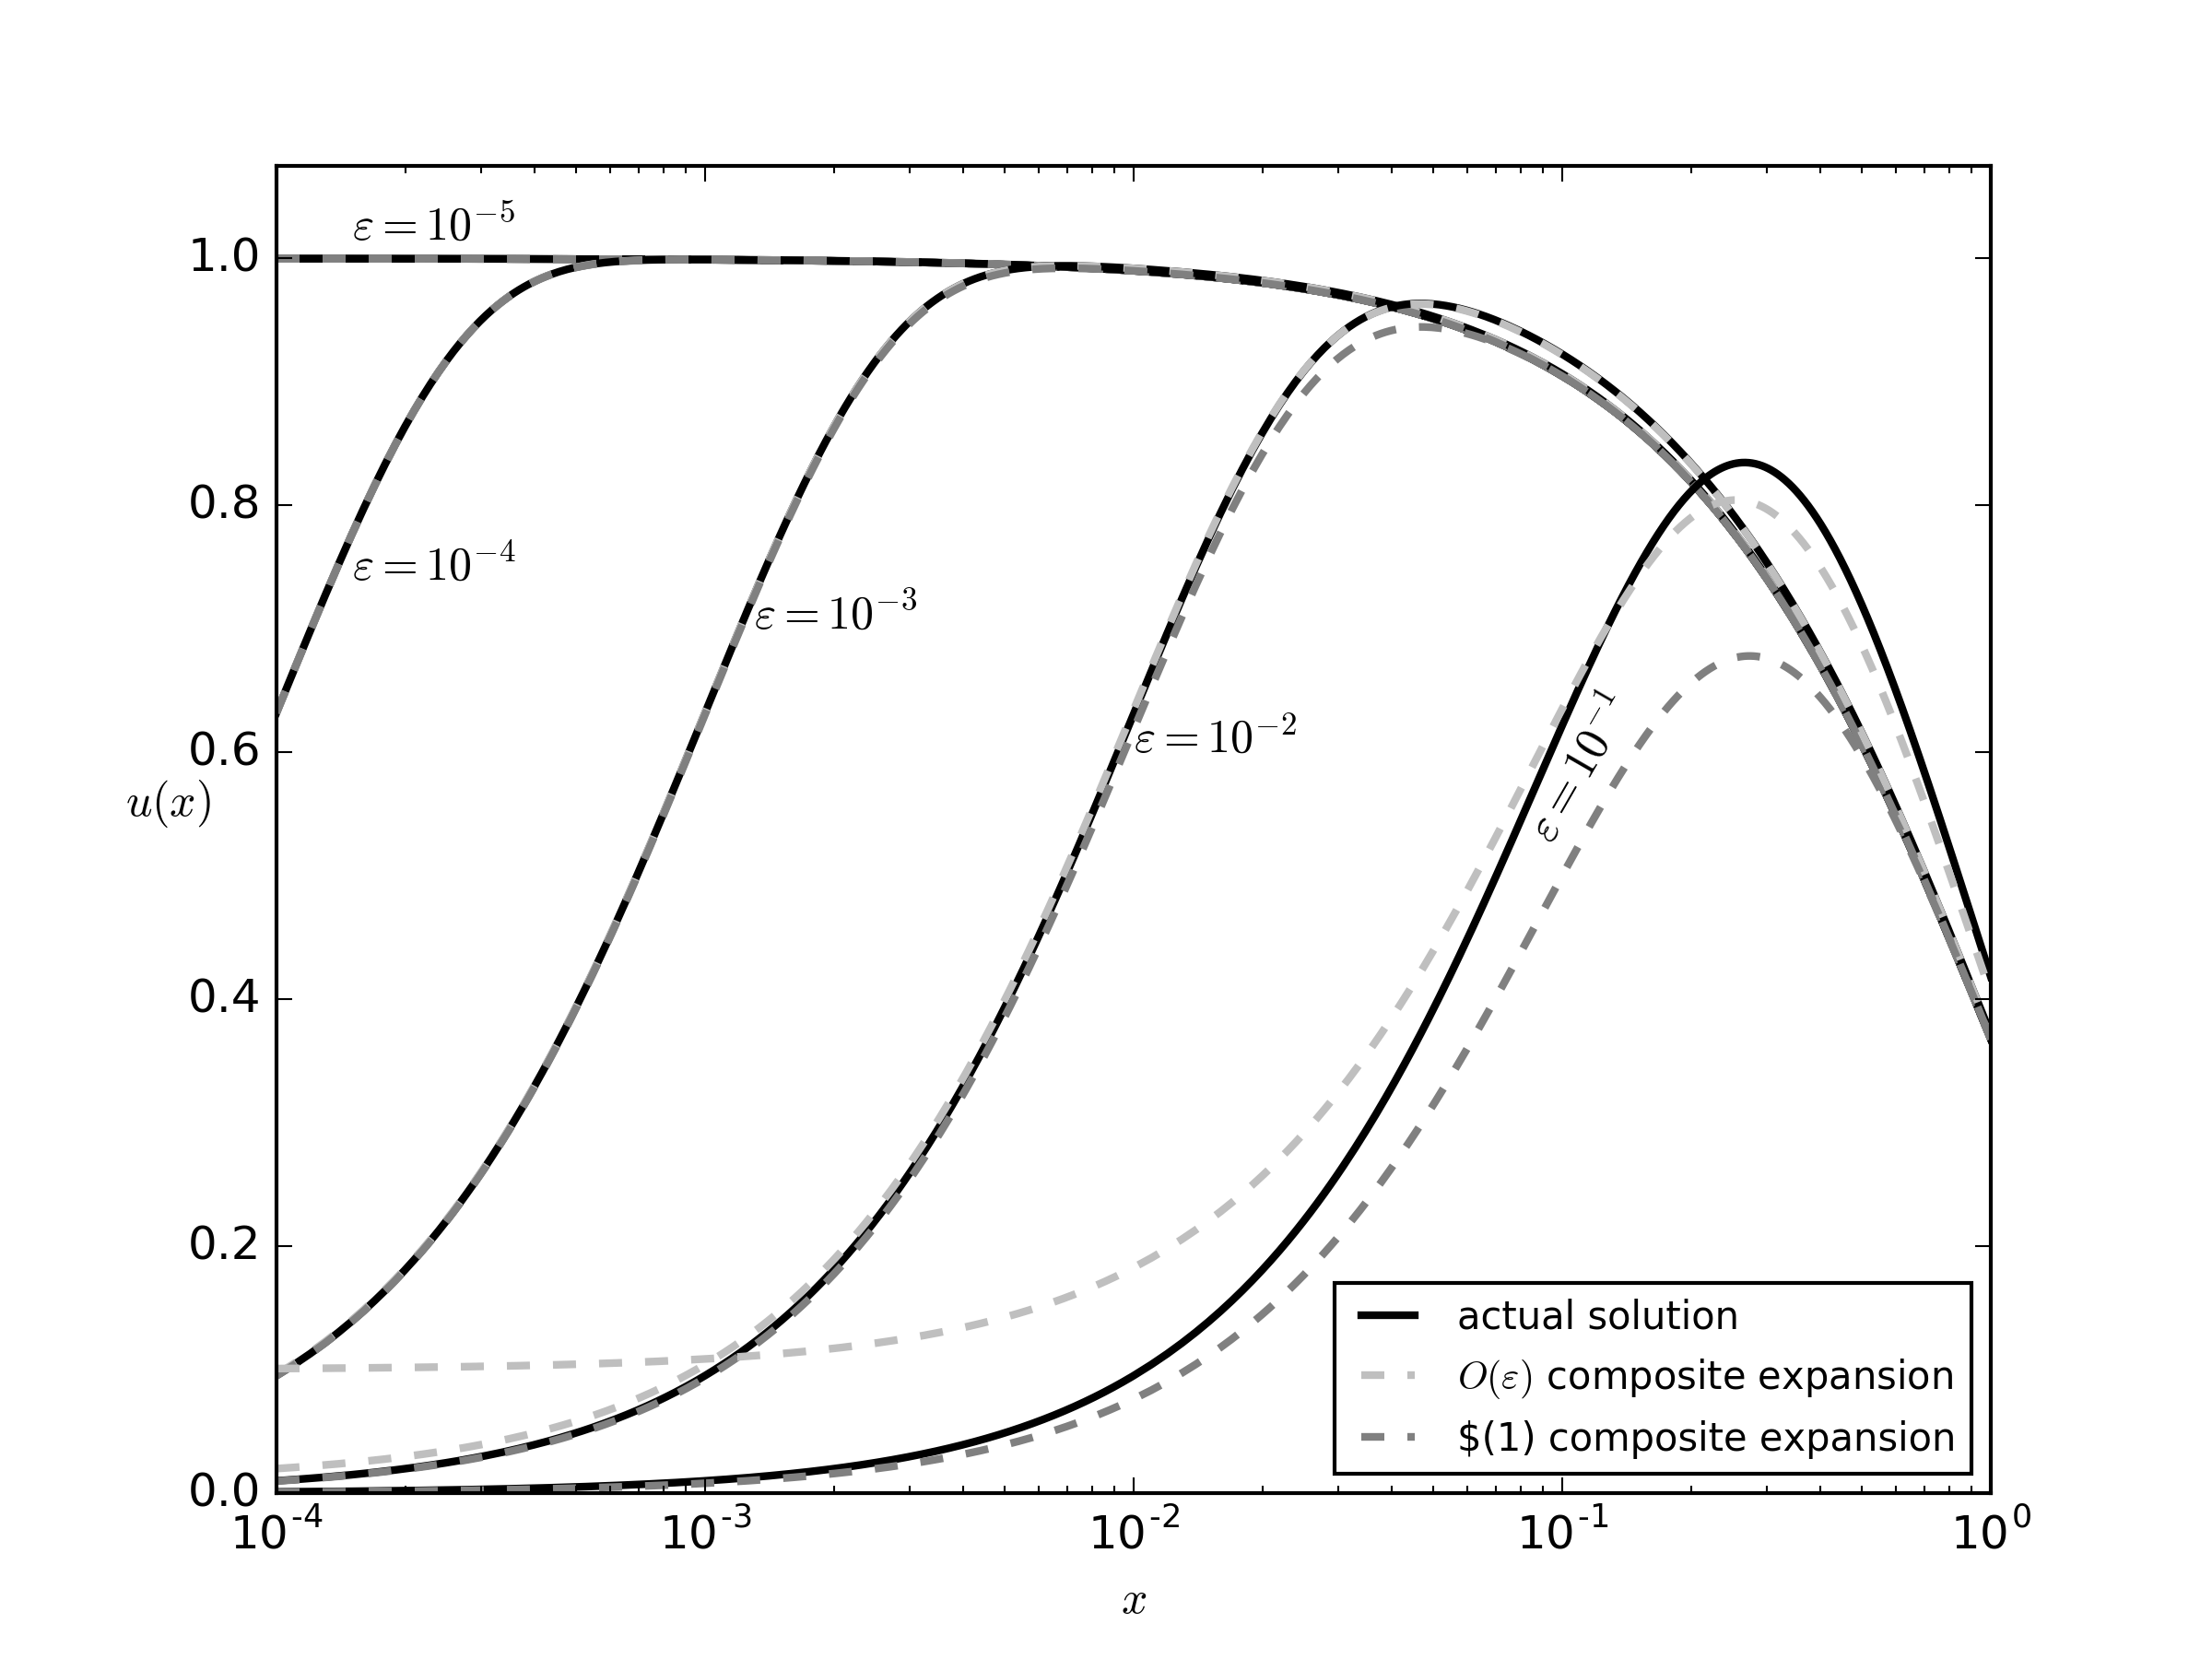
\includegraphics[width=0.75\textwidth]{semilog.png}\vspace{-0.22cm}
        \caption{The first two graphs show the actual solutions and composite expansions between $0$ and $1$ for $\E = 10^{-k}$ for $k = 1, 2, 3, 4, 5$ (\emph{calculated and plotted using Python 2.7}).}
        \label{problem_1_graphs}
    \end{figure}
    \begin{figure}
        \centering
        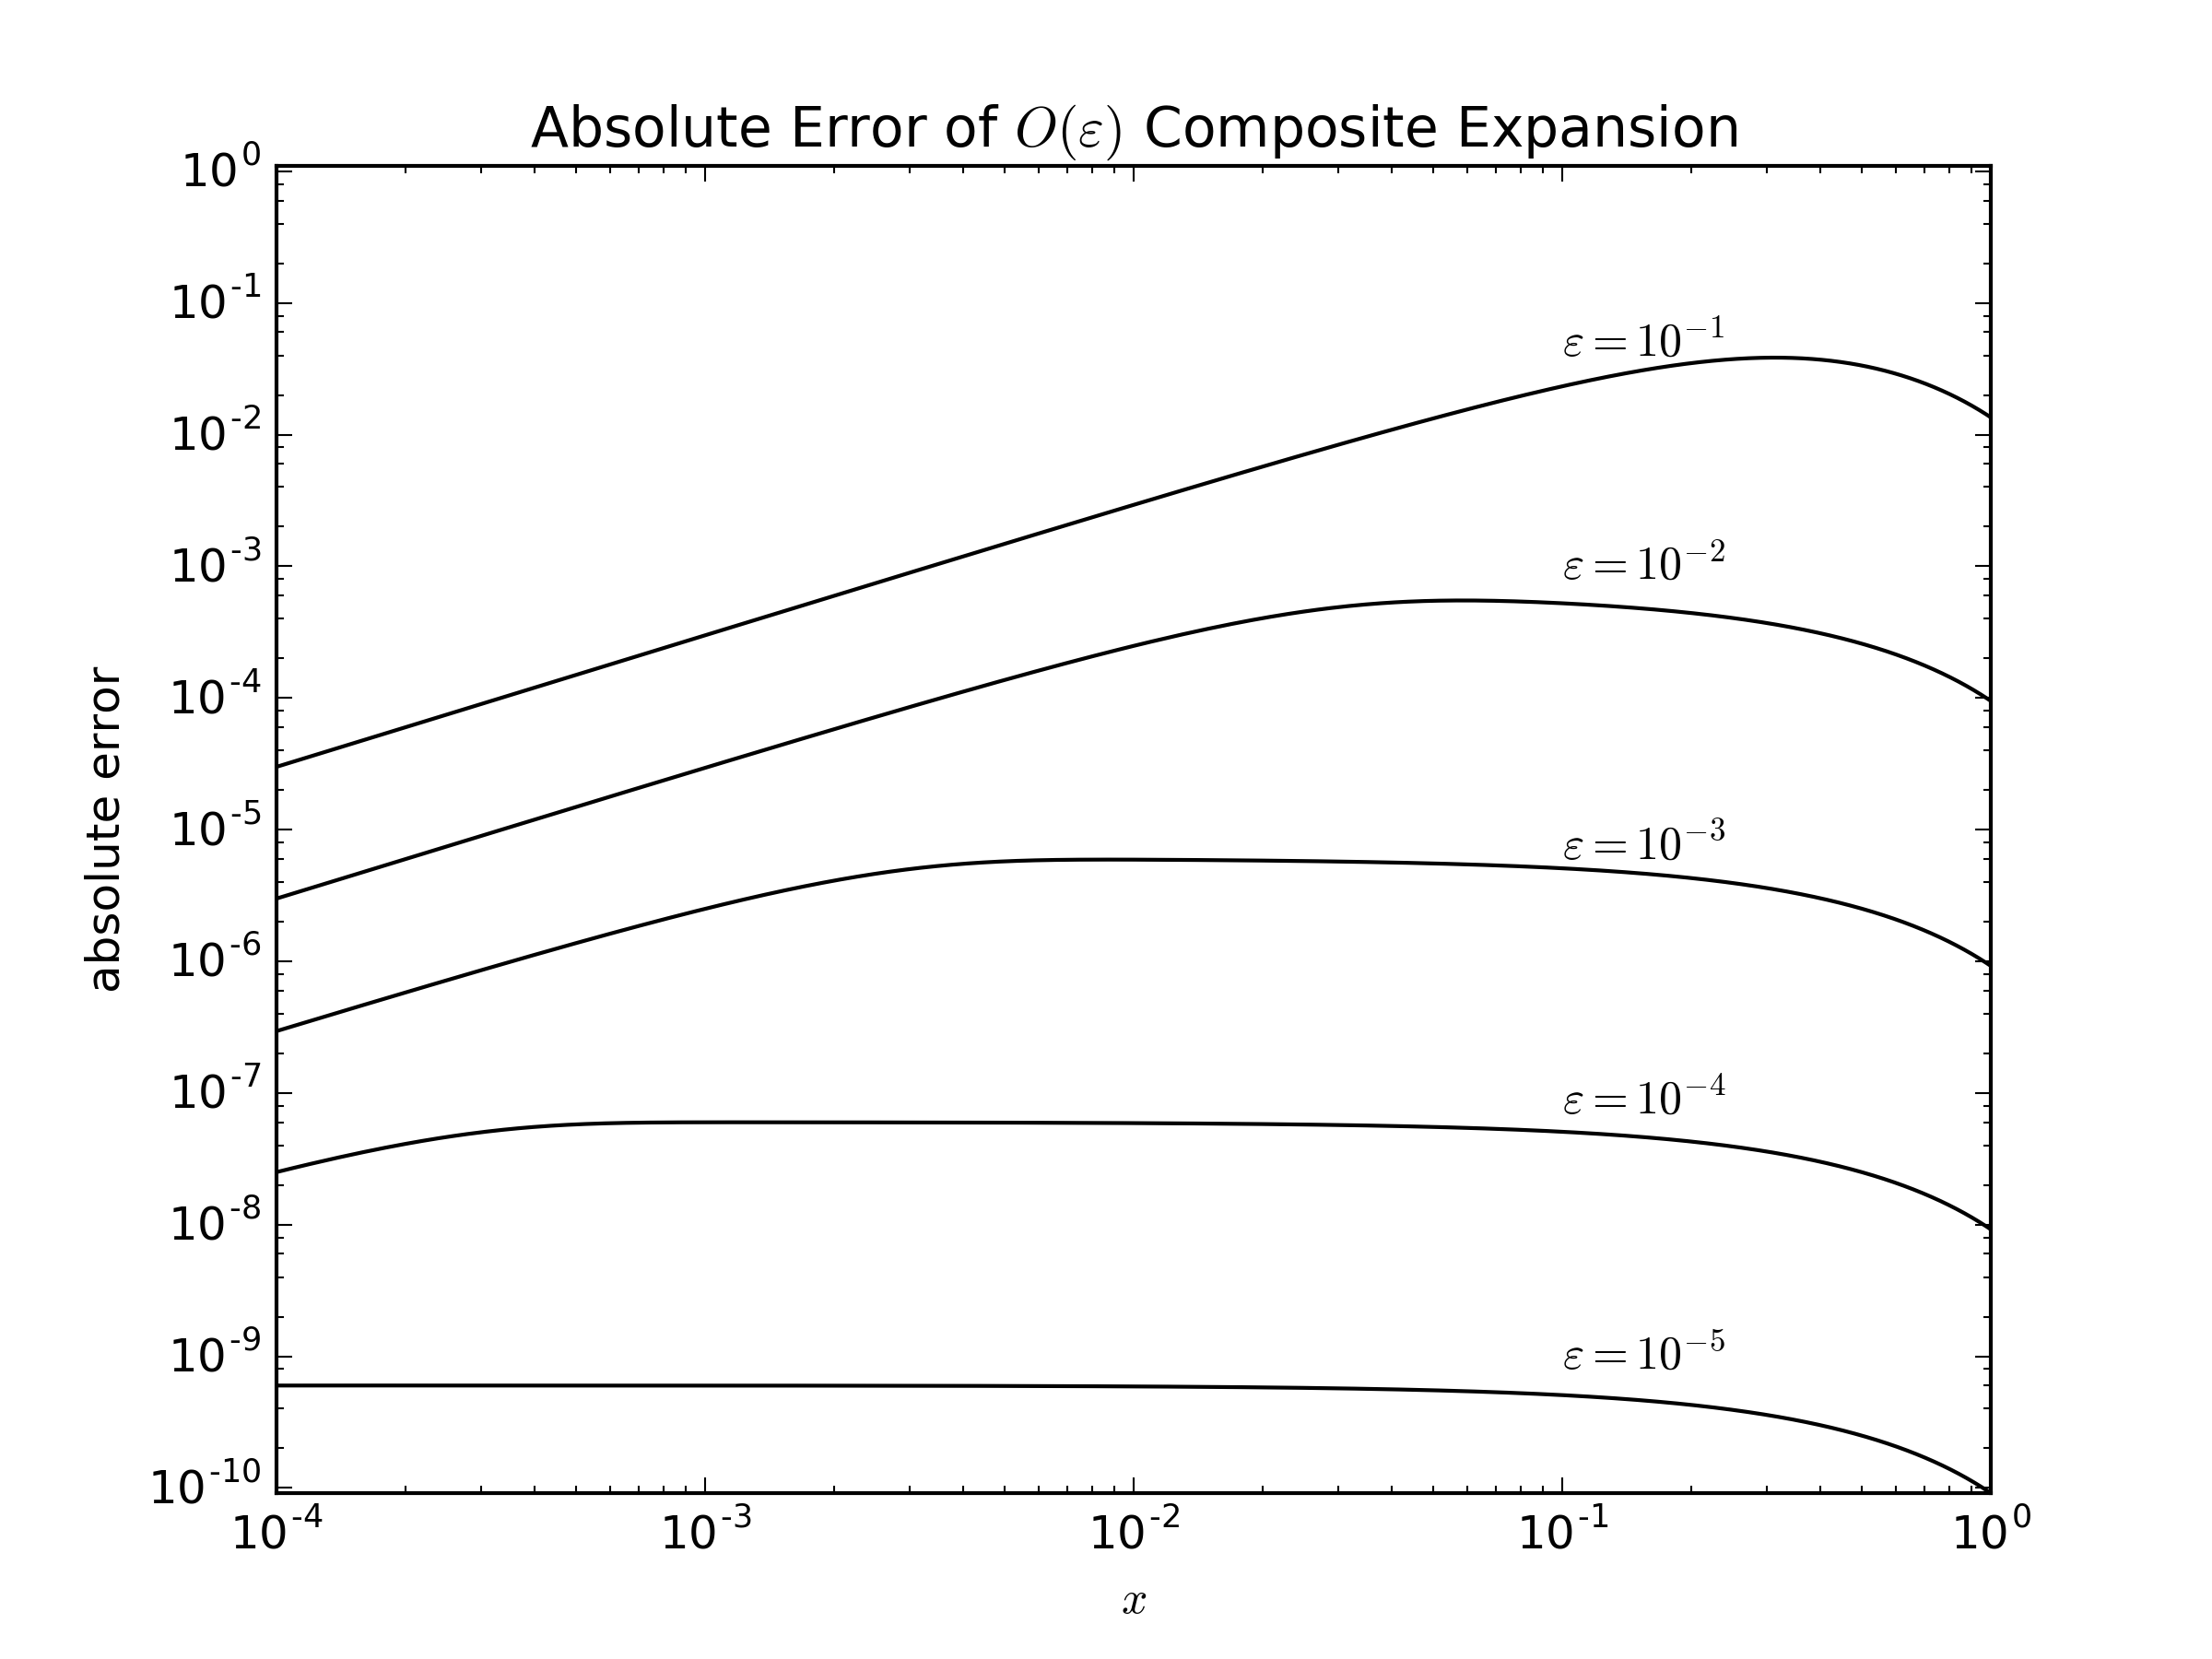
\includegraphics[width=0.75\textwidth]{errors_epsilon.png}\vspace{-0.22cm
        }
        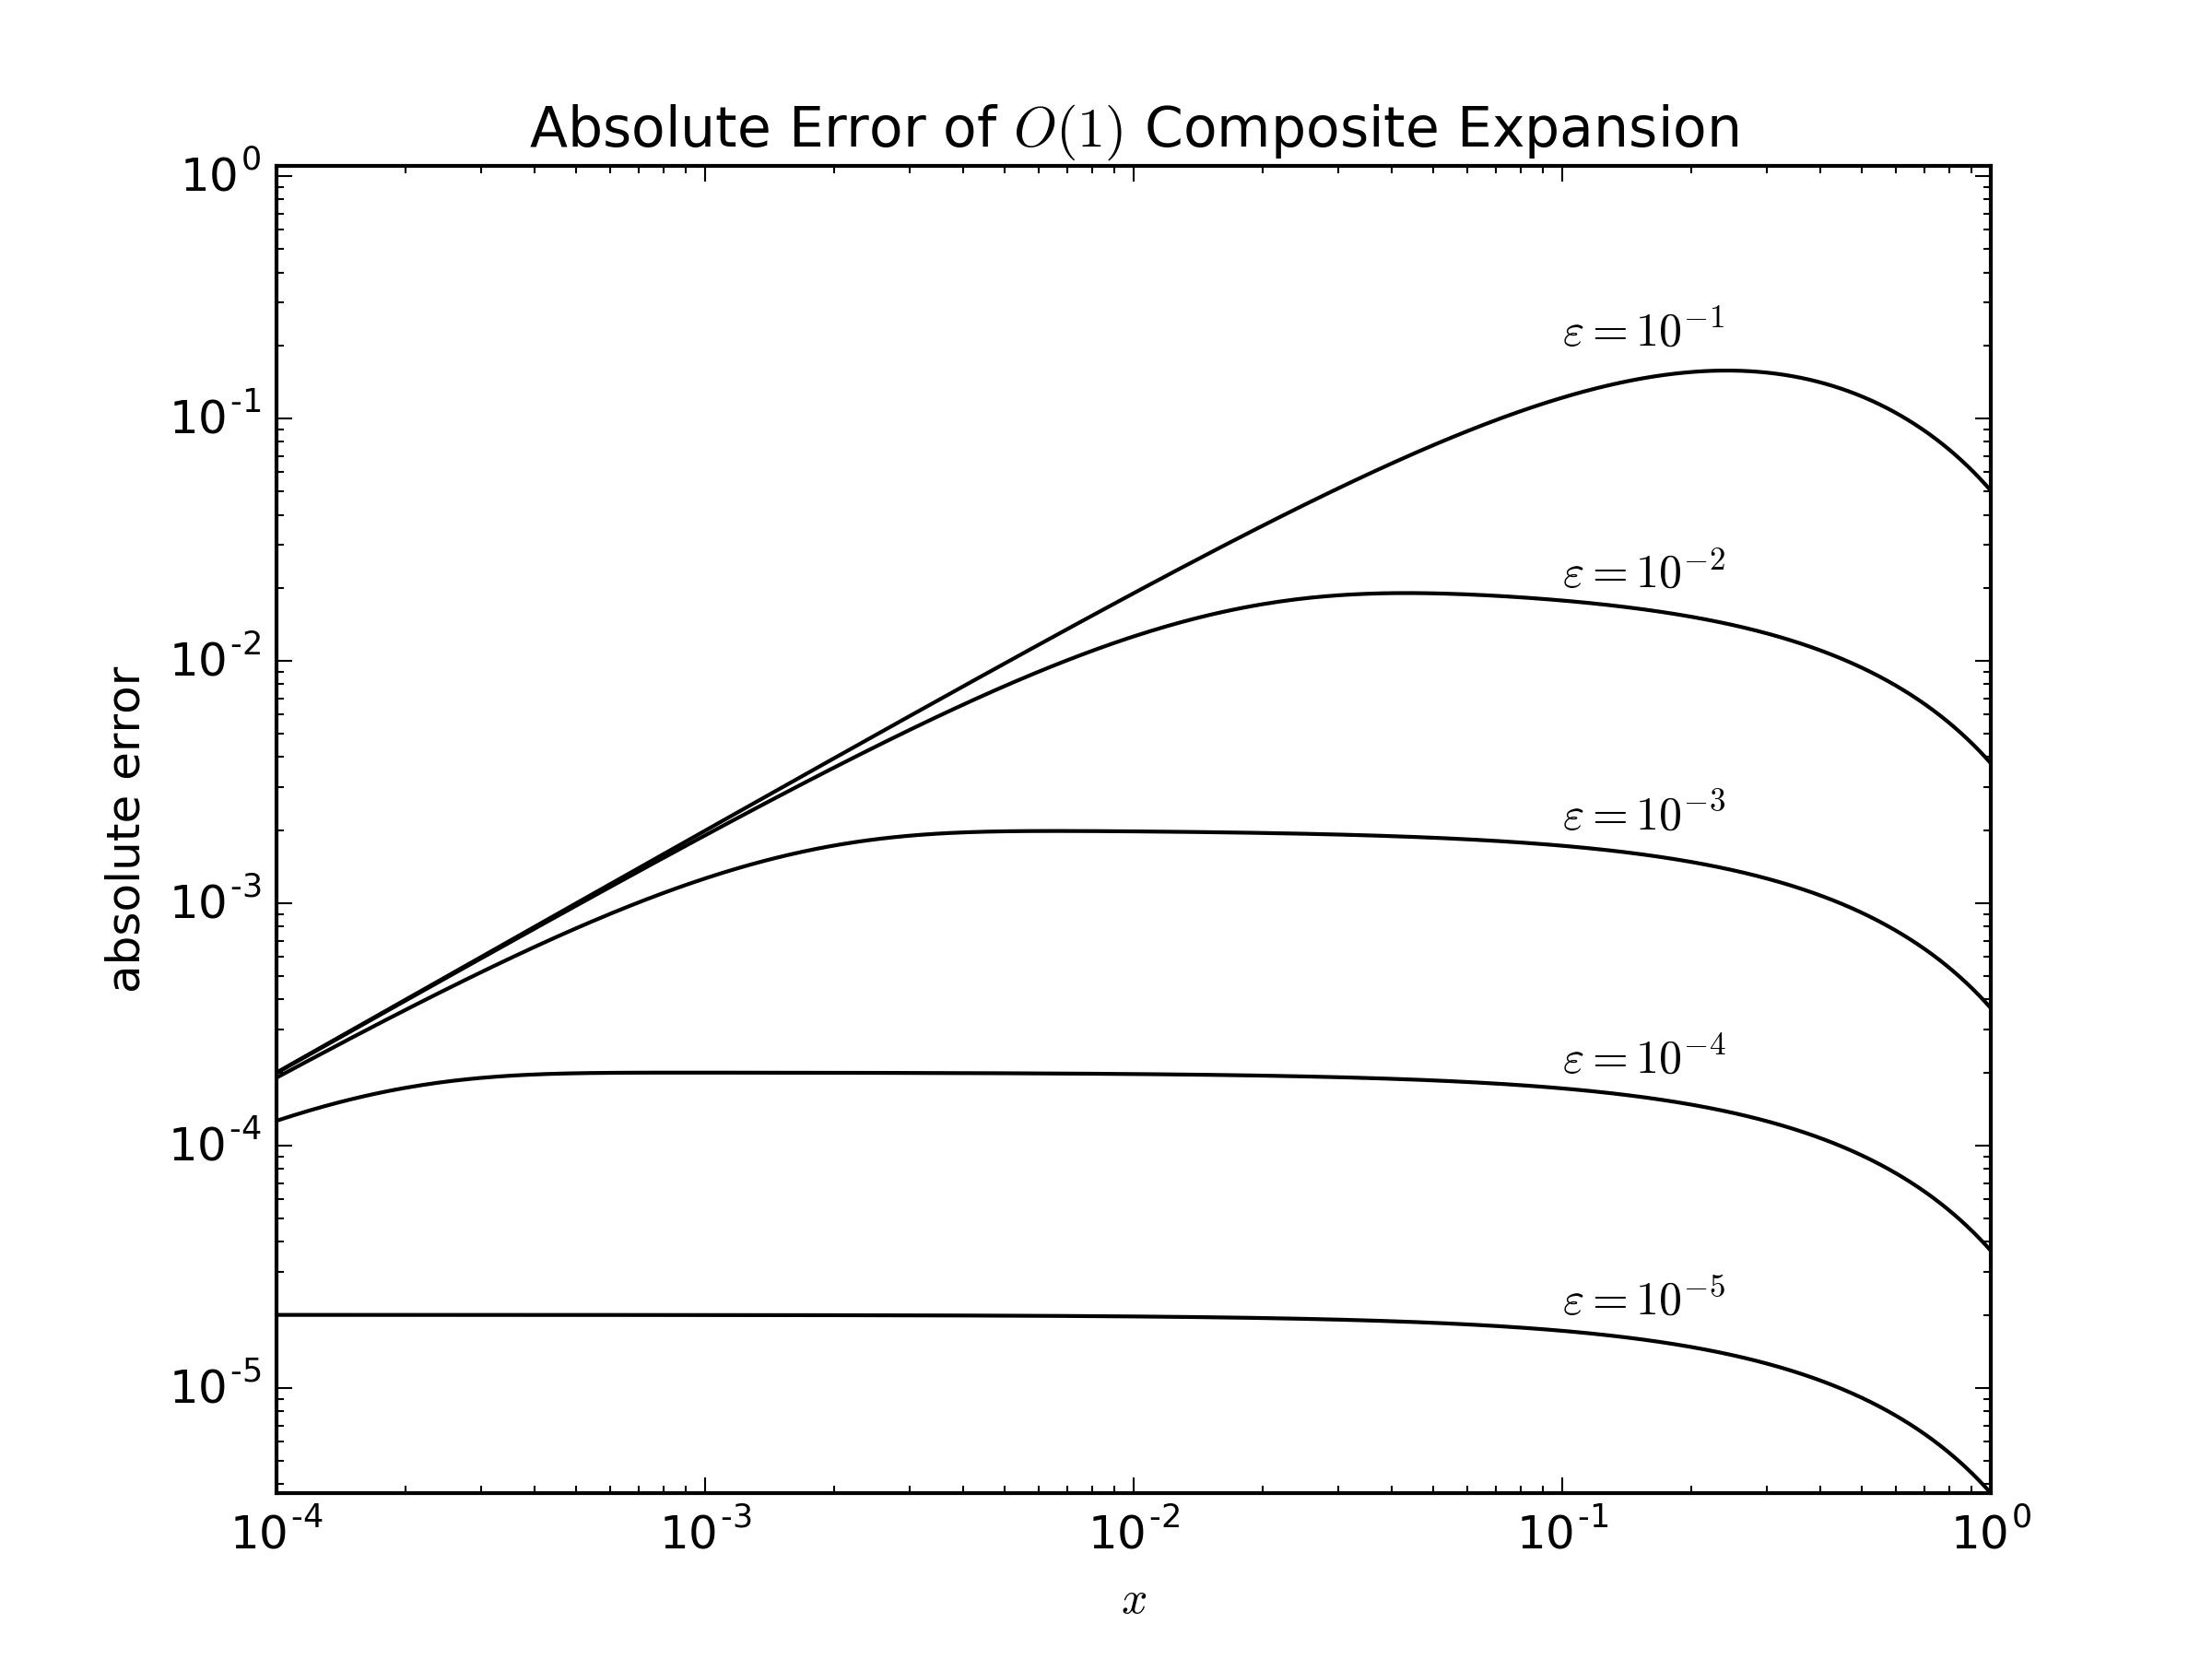
\includegraphics[width=0.75\textwidth]{errors_1.png}\vspace{-0.22cm}
        \caption{The two graphs show the aboslute errors between the actual solutions and composite expansions for $\E = 10^{-k}$ for $k = 1, 2, 3, 4, 5$ (\emph{calculated and plotted using Python 2.7}).}
        \label{problem_1_graphs_errors}
    \end{figure}
\end{proof}







\pagebreak
%%%%%%%%%%%%%%%%%%%%%%%%%%%%%%%%%%%%%%
\problem{Problem 2}{Compute the leading order composite expansion to the problem
\begin{align*}
    \E u'' + \sqrt{x}u' - u &= 0, \\
    u(0) = 0, \qquad u(1) &= e^2.
\end{align*}}
\begin{proof}
    First let $X = \frac{x - x_0}{\E^\alpha}$ and $U(X) = u(x)$.  Then $x = x_0 + \E^\alpha X$ and
    \begin{align*}
        \E \ddot{U} + \sqrt{x_0 + \E^\alpha X}\E^\alpha \dot{U} - \E^{2\alpha} U = 0
    \end{align*}
    There are three possibilities in matching two of these three terms in $\E$ order: $\alpha = 1, 0, \frac{1}{2}$.  $\alpha = \frac{1}{2}$ does not work since the term not matched is lower order than the others.  $\alpha = 0$ is the original problem, and so the only choice is $\alpha = 1$.  Then
    \begin{align*}
        \ddot{U} + \sqrt{x_0 + \E X}\dot{U} - \E U = 0
    \end{align*}
    Assuming $U = U_0 + U_1 \E + U_2 \E^2 + \dots$, then the $O(1)$ expansion ($U_0$) gives
    \begin{align*}
        \ddot{U}_0 + \sqrt{x_0}\dot{U}_0 = 0 \\
        \implies U_0 = A + Be^{-\sqrt{x_0}X}.
    \end{align*}
    This forces $x_0 = 0$, and thus the equation
    \begin{align*}
        \E \ddot{U} + \sqrt{x_0 + \E^\alpha X}\E^\alpha \dot{U} - \E^{2\alpha} U = 0 \\
        \E \ddot{U} + \sqrt{X}\E^{\frac{3\alpha}{2}} \dot{U} - \E^{2\alpha} U = 0
    \end{align*}
    Now there are three different $\alpha$ possibilities to match two of the three terms: $\alpha = 0, \frac{1}{2}, \frac{2}{3}$.  $\alpha = 0$ is the original problem, $\alpha = \frac{1}{2}$ does not work since the term not matched is lower order than the others, and so the only choice is $\alpha = \frac{2}{3}$.
    \begin{align*}
        \E \ddot{U} + \E \sqrt{X}\dot{U} - \E^{\frac{4}{3}}U = 0 \\
        \implies \ddot{U} + \sqrt{X}\dot{U} - \E^{\frac{1}{3}}U = 0 \\
    \end{align*}
    Assume $U = U_0 + \E U_1 + \E^2 U_2 + \dots$.  Then setting $\E \rightarrow 0$ yields
    \begin{align*}
        \ddot{U_0} + \sqrt{X}\dot{U_0} = 0 \qquad \implies \qquad U_0(X) = \int_0^X \qty[C\exp[-\frac{2}{3}T^{\frac{3}{2}}]]\dd T \qquad \implies \qquad u_\text{in}(x) \approx \int_0^{x\E^{-\frac{2}{3}}}\qty[C\exp[-\frac{2}{3}T^{\frac{3}{2}}]]\dd T
    \end{align*}
    The original outer problem is
    \begin{align*}
        \E \ddot{u} + \sqrt{x}\dot{u} - u = 0, \qquad u(0) = 0
    \end{align*}
    Assuming $u = u_0 + \E u_1 + \E^2 u_2 + \dots$,
    \begin{align*}
        \sqrt{x}\dot{u}_0 - u_0 = 0, \qquad u_0(1) = e^2
    \end{align*}
    which has the solution
    \begin{align*}
        u_0(x) = e^{2\sqrt{x}} \qquad \implies \qquad u_{\text{out}}(x) \approx e^{2\sqrt{x}}
    \end{align*}
    To match $u_\text{in}$ with $u_\text{out}$, we want
    \begin{align*}
        \lim_{x \rightarrow 0} u_\text{out} &= \lim_{x \rightarrow \infty} u_\text{in} \\
        \lim_{x \rightarrow 0} e^{2\sqrt{x}} &= \lim_{x \rightarrow \infty} \int_0^{x\E^{-\frac{2}{3}}}\qty[C\exp[-\frac{2}{3}T^{\frac{3}{2}}]]\dd T \\
        1 &= \int_0^\infty \qty[C\exp[-\frac{2}{3}T^{\frac{3}{2}}]]\dd T \\
        \implies C &= \frac{1}{\displaystyle\int_0^\infty \qty[\exp[-\frac{2}{3}T^{\frac{3}{2}}]]\dd T}.
    \end{align*}
    Also, this says $u_\text{match} = 1$ (since $u_{\text{match}} = \lim_{x \rightarrow 0} u_{\text{out}} = \lim_{x \rightarrow \infty} u_{\text{in}} = 1$).
    Thus,
    \begin{align*}
        u(x) &\approx u_\text{in}(x) + u_\text{out}(x) - u_\text{match}(x) \\
        &= e^{2\sqrt{x}} + \displaystyle\frac{\displaystyle\int_0^{x\E^{-\frac{2}{3}}}\qty[\exp[-\frac{2}{3}T^{\frac{3}{2}}]]\dd T}{\displaystyle\int_0^\infty\qty[\exp[-\frac{2}{3}T^{\frac{3}{2}}]]\dd T} - 1
    \end{align*}
\end{proof}








\end{document}
